\documentclass[11pt]{article}
\usepackage{amsmath, amssymb, amsthm}
\usepackage[retainorgcmds]{IEEEtrantools}

\usepackage{tikz}
\usetikzlibrary{intersections, decorations.pathreplacing}

\usepackage{fancyhdr}

%Format stuff
\pagestyle{fancy}
\headheight 35pt

%Header info
\chead{\Large \textbf{Greedy Scheduling Algorithms}}
\lhead{}
\rhead{}

\begin{document}

\section{Interval Scheduling}

	\begin{description}
		\item[Input:] A set of requests $R$ for a resources, where $\forall r \in R$, there is a start time $s_i$ and finish time $f_i$.
		\item[Output:] A subset of $R$ with no conflicts that maximizes the number of scheduled events.
	\end{description}
	
	\subsection{Greedy Criterion}
		A number of schemes are possible for the algorithm, including shortest request first, earliest start time first, and earliest finish time first.
		
		Shortest request is suboptimal from the following counterexample, where it would schedule two requests instead of the optimal 3. By extrapolating this principle, shortest request could be off by a factor of 2 from the optimal schedule because one request can conflict with 2 optimal requests.
		\begin{center}
		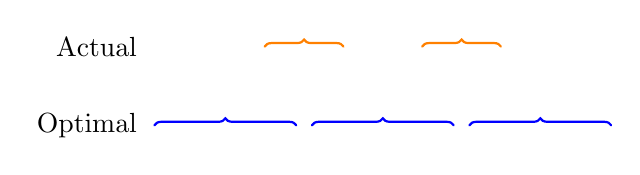
\begin{tikzpicture}
			[scale=1,line cap=round,
			%Styles
			axes/.style=,
			important line/.style={very thick},
			information text/.style={rounded corners,fill=red!10,inner sep=1ex},
			dot/.style={circle,inner sep=1pt,fill,label={#1},name=#1}			
			]
			
			%Colors
			\colorlet{anglecolor}{green!50!black}	%angle arcs/lines
			
			%The graphic
			
			\node[left] at (0, 0) {Actual};
			\node[left] at (0, -1) {Optimal};
			
			\draw[decorate,decoration=brace,blue,thick] (.1, -1) -- (1.9, -1);
			\draw[decorate,decoration=brace,blue,thick] (2.1, -1) -- (3.9, -1);
			\draw[decorate,decoration=brace,blue,thick] (4.1, -1) -- (5.9, -1);
			
			\draw[decorate,decoration=brace,orange,thick] (1.5, 0) -- (2.5, 0);
			\draw[decorate,decoration=brace,orange,thick] (3.5, 0) -- (4.5, 0);
		\end{tikzpicture}
		\end{center}
		
		Earliest start time is actually a horrible criterion, as demonstrated by the following counterexample:
		
		\begin{center}
		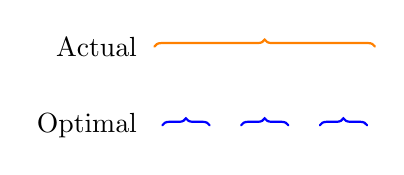
\begin{tikzpicture}
			[scale=1,line cap=round,
			%Styles
			axes/.style=,
			important line/.style={very thick},
			information text/.style={rounded corners,fill=red!10,inner sep=1ex},
			dot/.style={circle,inner sep=1pt,fill,label={#1},name=#1}			
			]
			
			%Colors
			\colorlet{anglecolor}{green!50!black}	%angle arcs/lines
			
			%The graphic
			
			\node[left] at (0, 0) {Actual};
			\node[left] at (0, -1) {Optimal};
			
			\draw[decorate,decoration=brace,blue,thick] (.2, -1) -- (.8, -1);
			\draw[decorate,decoration=brace,blue,thick] (1.2, -1) -- (1.8, -1);
			\draw[decorate,decoration=brace,blue,thick] (2.2, -1) -- (2.8, -1);
			
			\draw[decorate,decoration=brace,orange,thick] (.1, 0) -- (2.9, 0);
		\end{tikzpicture}
		\end{center}
		
		In the end, the optimal greedy criterion is actually sorting requests by earliest finish time, because it frees up the shared resource ASAP. Note this can be implemented in $\Theta(n)$ time by one walkthrough of the list - pick the first valid element, then walk along the list until the next valid start time, and so on.
		
	\subsection{Proof}
		Let $O$ be some optimal schedule and $G$ be the greedy schedule generated by the algorithm such that $O = G$ up to some index $j$. From our greedy criterion, we know that $f_j^G \leq f_j^O$. Therefore, we can swap $O_j$ with $G_j$ without introducing any more conflict, producing a new still-optimal schedule $O'$.
		
		By induction, it is possible to transform any optimal schedule into our greedy schedule while maintaining optimality. Therefore, the greedy algorithm produces an optimal schedule.

\section{Cache Scheduling}
	\begin{description}
		\item[Input:] A list of jobs $j$ each with a weight $w_j$ and length $l_j$.
		\item[Output:] An ordering of jobs that minimizes the weighted sum of completion times, where completion time is the amount of wall time it takes from the beginning to the completion of job $j$.
		\[C_j = \sum_1^j l_j\]
		\[min(\sum_1^nw_jC_j)\]
	\end{description}
	
\subsection{Greedy Criterion}
	\subsubsection{Special Cases}
		\subparagraph{Identical lengths} In this case, we choose the larger-weight jobs first to minimize the term in the sum (when $n$ is smaller).
			\begin{equation}
				\sum_1^n w_jC_j = \sum_1^n w_j \cdot n \cdot L = L \cdot \sum_1^n w_j \cdot n
			\end{equation}
		\subparagraph{Identical weights} In this case, we choose the shortest jobs first to minimize the sum over completion times.
			\begin{equation}
				\sum_1^n WC_j = W\sum_1^n C_j
			\end{equation}
			
	\subsubsection{Resolving Conflicting Advice}
		The key idea is to assign each job a score that is directly proportional with $w$ and indirectly proportional with $l$. Taking two guesses at such a score, there are 
		\begin{itemize}
			\item $s_j = w_j - l_j$
			\item $s_j = w_j / l_j$
		\end{itemize}
		To distinguish between the two, find the simplest example that produces different outputs. In this case, for the two jobs $j_1(w=3, l=5), j_2(w=1,l=2)$, the second score yields the lower weighted sum, so it is better than the first.
		
\section{Proof}
	\begin{description}
		\item[Claim:] sorting by decreasing ratio $w_j / l_j$ is always correct
		\item[Proof:] by exchange argument and contradiction.
		\item[Assume:] no ties in ratios (doesn't change algorithm, only proof)
	\end{description}
	
	Fix an arbitrary input of $n$ jobs with $\sigma$ as the greedy schedule from the algorithm and $\sigma^*$ being a theoretically optimal algorithm. Next, rename the jobs $j_1, j_2, \ldots , j_n$ such that $s_1 > s_2 > \ldots > s_n$, so that $\sigma$ just involves ordering the jobs in numerical order.
	
	Assuming $\sigma^* \neq \sigma$, there must exist two consecutive jobs $(i, j) \in \sigma^* \mid i > j$. Because $\sigma$ is a unique schedule (properly ordered), the only way $\sigma^*$ can be different is if at least one pair of jobs is flipped.
	
	Suppose we exchange the order of these two jobs in $\sigma^*$, leaving all other jobs unchanged. Jobs other than these two have no impact on completion time after this operation, while $C_i$ increases and $C_j$ decreases.
	
	\begin{IEEEeqnarray}{rCl}
		i > j & \rightarrow & \frac{w_i}{l_i} < \frac{w_j}{l_j}\\
		&& w_i l_j < w_j l _i
	\end{IEEEeqnarray}
	
	From the definition of weighted sum, it's clear that the cost associated with this exchange is outweighed by the benefit. Therefore, it is impossible for $\sigma^*$ to be optimal, violating out assumption in the first step, so $\sigma$ is an optimal schedule.
%	\begin{center}
%	\begin{tikzpicture}
%		[scale=3,line cap=round,
%		%Styles
%		axes/.style=,
%		important line/.style={very thick},
%		information text/.style={rounded corners,fill=red!10,inner sep=1ex},
%		dot/.style={circle,inner sep=1pt,fill,label={#1},name=#1}			
%		]
%		
%		%Colors
%		\colorlet{anglecolor}{green!50!black}	%angle arcs/lines
%		
%		%The graphic
%	\end{tikzpicture}
%	\end{center}

%	\begin{figure}[htb]
%		\centering
%		\includegraphics[width=0.8\textwidth]{filename.eps}
%		\caption{Caption.}
%		\label{fig:figure}
%	\end{figure}

%		\def\enotesize{\normalsize}
%		\theendnotes
\end{document}